\chapter{Background}

The study of networks is common across several scientific disciplines, including computer science, mathematics, physics, biology, statistics and sociology. In order to effectively study and work with this data, a general understanding of the concepts of graph theory and complex networks is required. This chapter serves as jumping off point for the computer science student looking to become for familiar with these critical definitions and concepts. This chapter also introduces the fundamentals of genetic algorithms, and the concept of optimization through population based meta-heuristics.

\label{system}
\section{Elements of Graph Theory}
A \textit{Graph G} is composed of two sets, (\textit{V,E}), where \textit{V} is the set of \textit{vertices}, or \textit{nodes} and \textit{E} is the set of unordered pairs of elements of \textit{V}. If these pairs are ordered, the graph is \textit{directed}. Elements of \textit{E} are referred to as edges. An edge connects two nodes. Nodes associated with a particular edge are called \textit{endpoints}. 
\begin{figure}[!h]
	\begin{center}
		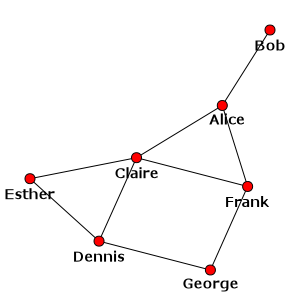
\includegraphics[scale=0.5]{images/simple_graph.png}
	\end{center}
	\caption{An undirected graph with 7 nodes and 9 edges.}
	\label{logo}
\end{figure}

A network can be visualized simply as nodes, drawn as points, connected by their corresponding edges. Note that graphs do not include self edges, called \textit{loops} or more than one edge joining the same pair of vertices. However, \textit{multigraphs} are a generalization which allow these constructs. 

A \textit{subgraph} of \textit{G = (V, E)} is denoted as \textit{$G^\prime$ = ($V^\prime$, $E^\prime$)} if \textit{$V^\prime$} $\subset$ \textit{V} and \textit{$V^\prime$} $\subset$ \textit{E}. A subgraph which contains edges such that all \textit{v}$\in$\textit{V} are endpoints is a \textit{spanning subgraph} of \textit{G}. 
A partition of a vertex set \textit{V} into two subsets \textit{S} and \textit{V $-$ S} is called a cut. The \textit{cut size} is the number of edges connecting members of \textit{S} to \textit{V $-$ S}
A \textit{path} is a finite set of edges that connect two vertices. If, for some vertices in \textit{G} no path exists, \textit{G} is a \textit{disconnected} graph.

The number of vertices and edges of a graph are indicated with \textit{n} and \textit{m}. \textit{n} is the order of a graph, and \textit{m} is the size. The maximum size of a graph if order \textit{n} is $n(n-1)/2$, the number of unordered pairs of vertices. If \textit{G} is of maximum size, each vertex having an edge to every other, it is a \textit{complete graph}. 
A fully connected subgraph is called a \textit{clique}. Endpoints are referred to as \textit{neighbors}, or \textit{adjacent nodes}. The the set of neighbors of vertex \textit{v} is the \textit{neighborhood}, indicated as \textit{$\Gamma(v)$}. $|\Gamma(v)|$, the number of neighbors of \textit{v}, is the degree of \textit{v}, $k_v$. The \textit{degree sequence} of $G$ is the list of degrees for each vertex of $G$, $k_{v1}, k_{v2},\dots, k_{vn}$. 
A regular graph is one whose degree sequence contains only copies of a single integer. Directed graphs distinguish between the \textit{indegree} and \textit{outdegree}, the number of edges ending at \textit{v}, and beginning at \textit{v} respectively. While in this paper we limit experiments to unweighted graphs, it is important to understand the extension of edges from being counted as binary entities, to ones with real values. These edge values are called \textit{weights}. The analog to degree of $v$ in these graphs is \textit{strength}, the sum of edge weights adjacent to $v$.


If a pair of vertexes are connected, the graph $P$, composed of the set of vertexes $V(P)=\{x_0, x_1,\dots, x_{l-1}, x_l\}$ and edges $E(P=\{(x_0,x_1), (x_1,x_2),\dots,(x_{l-1}, x_{l})\})$. The vertices $x_0$ and $x_l$ are connected by the set of %%TODO

The \textit{internal degree} and \textit{external degree}, $k^{int}_i$ and $k^{ext}_i$, with respect to node $i$ being a member of subgraph $C\subset G$, are the sum of edges connecting $i$ to nodes in $C$ and not contained in $C$ respectively. 
Another useful measure on vertices is \textit{clustering} \cite{Watts1998}, or \textit{transitivity} to avoid confusion when dealing with structural clusters. $C_v$, the transitivity of $v$, is the ratio of edges joining pairs of nodes in $\Gamma(v)$, to the total possible number of edges between nodes in $\Gamma(v)$. For node $v$, the transitivity is given as: $$k_v(k_v-1)/2$$ Another way of expressing the transitivity is in the number of triangles formed with $v$. Note that the clustering value of a graph does not measure how a graph may be partitioned directly, as it correlates with the size and volume of the network \cite{Kunegis2013}. Instead, it can be used as a normalized value to compare different networks in terms of how many triangles exist per node.

A common mathematical procedure to apply to graphs is a \textit{random walk}. As the name implies, it is  randomly generated set of steps along a path. Given a node, selected as the starting point, each step is making the transition from the current node $i$, to the next node $j$, given that $j\in\Gamma{i}$ with the probability $\frac{1}{k_i}$. Random walks have varied applications to problems in graph theory, and are a common feature of community detection methods \cite{Pons2006}.




\subsection{The Adjacency Matrix}
When dealing with graphs, one of the most effective ways to represent their structure, or \textit{topology}, is an \textit{adjacency matrix}. For a binary graph $G$, its adjacency matrix is an $n\times n$ matrix $A$. Where nodes $i$ and $j$ share an edge, $A_{ij}$ is 1, and otherwise 0. This matrix is symmetric in the case of undirected graphs. The sum of the $i$-th row of $A$ is the degree of node $i$.
When The graph is weighted, it is indicated as $W$, where the element $W_{ij}$ is the weight of the edge connecting adjacent nodes $i$ and $j$.

\section{Complex Networks}
The great numbers of applications of graph theory have made it one of the foundational concepts in several fields. With this abundance of interest, a shift has occurred away from understanding local properties in small graphs, to understanding the statistical properties of large systems. Graphs of natural systems do not follow the same patterns as regular or random graphs, instead exhibiting a mix of properties which show both order and noise. Natural systems are organized %% TODO

\section{Properties of Networks}
%%TODO

\subsection{The Small World Effect}

A frequent observation in networks is the fact that most nodes are not in each others neighborhood, the distance most pairs of nodes is fairly small. Formally, they are defined as a network where the average path between any two nodes is scaled by the logarithm of th number of nodes.

\subsection{Scale Free Networks}

In regular graphs, the degree distribution is relatively consistent, with very little deviation from the average. In random models, the distribution is related to the probability of linkage. Real world networks rarely, if ever, show these features.


Figure \ref{power} shows the degree distributions of a random graph with 1000 nodes and a linkage probability of 0.01, and for a network of protein interactions in yeast. Many real networks show a similar property; the average degree is low, but there is a long tail to the distribution reaching far above the average. This manifests visually as dense hubs. One of the early observations of this fact was made in studies of citations of papers. Most are cited only a few times, while seminal publications are widely cited as the basis of many branching works. When the degree distribution is plotted, the tail of the graph extends t.

\begin{figure}[!h]
	\title{wat}
	\begin{center}
		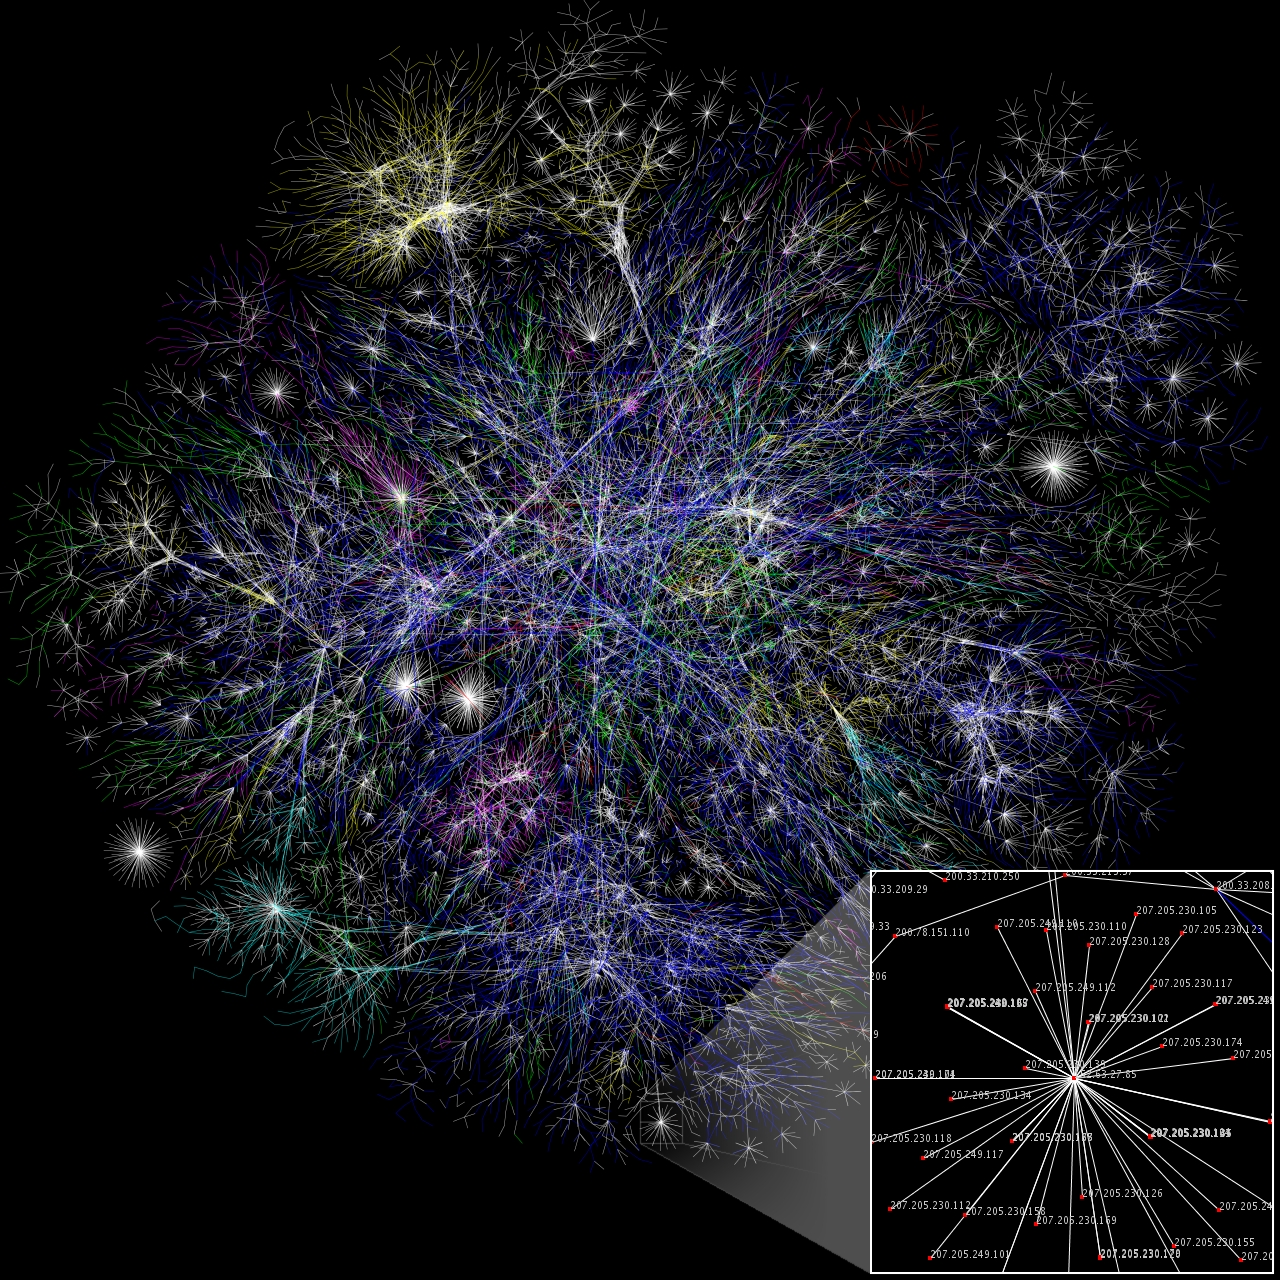
\includegraphics[scale=0.15]{images/Internet_map_1024.jpg}
	\end{center}
	\caption{A section of the Internet, as represented by the Opte Project in 2005.}
	\label{opte}
\end{figure}


\begin{figure}
	\begin{tabular}{cc}
		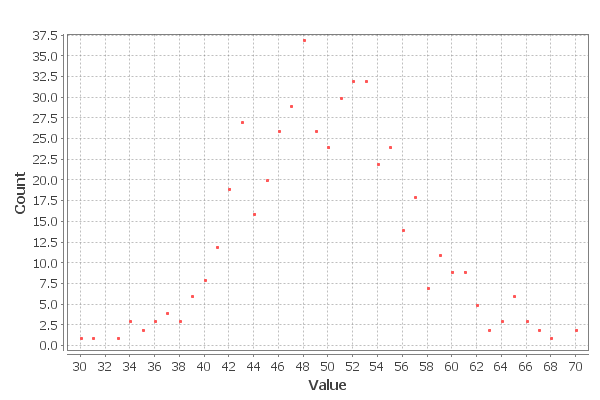
\includegraphics[width=65mm]{images/random-degree-distribution.png} &   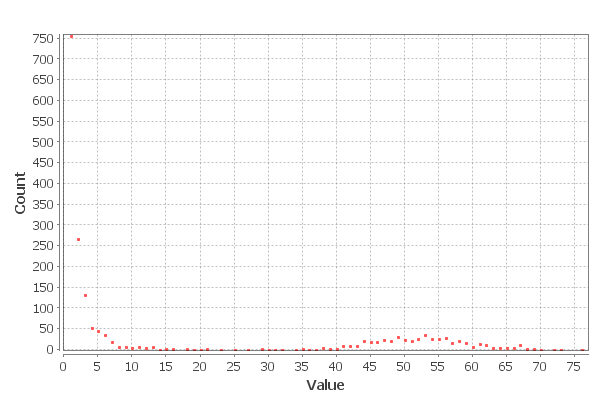
\includegraphics[width=65mm]{images/yeast-degree-distribution.png} \\
		(a) Random Network & (b) Yeast \\[6pt]
	\end{tabular}
	\caption{The degree distribution of a random network of 1000 nodes (a), and of a network of protein interactions in yeast\do}
	\label{power}
\end{figure}


\section{Community Detection In Graphs}
When visualizing real world networks, it is common to see some structure in the noise. In social graphs, these may be close friend groups. In collaboration networks, groups of researchers may interact closely to those in related fields, but rarely with those more removed from their areas of interest. These \textit{communities} can offer a better understanding to how the network is organized, and how these modules may or may not interact. It gives researchers a way to identify smaller sections of interest in networks for closer study. It offers a method to classify nodes based on their role, or relationship to the structure.
\begin{figure}[!h]
	\begin{center}
		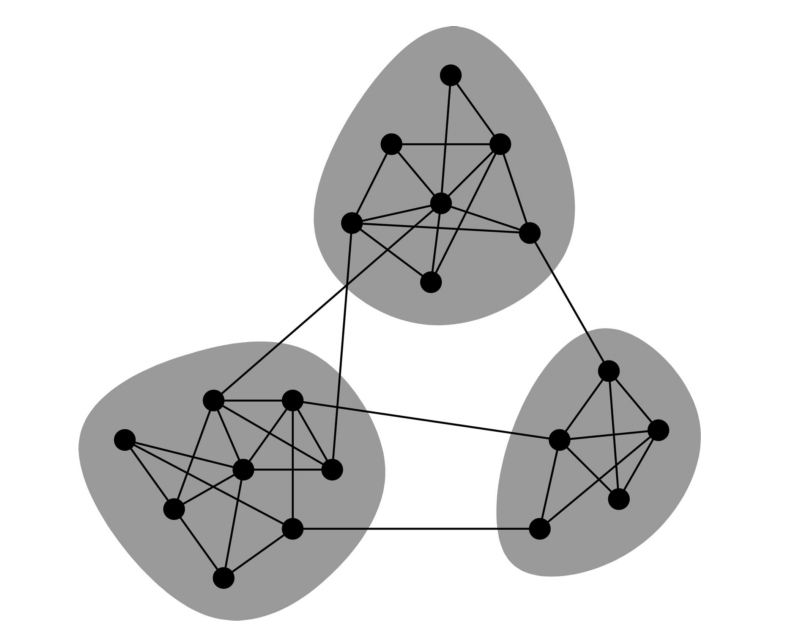
\includegraphics[scale=0.7]{images/communities.png}
	\end{center}
	\caption{Each shaded area of the graph is a community component}
	\label{logo}
\end{figure}


The identification and study of community structure has three major roles \cite{Lancichinetti2010}. First, it shows the organization of the graph at a courser level, as if its functional units were compressed. This understanding can allow for better insights into how the network was built, and how it may continue to evolve as a system. Secondly, it helps better explain dynamic processes as the take place. Examples like the spread of disease, or ideas over social media are considerably affected by the modular structure of the components of the system. Finally, it provides insight into relationships between entities of the system, which may not be apparent when viewing the system as a whole. 

\subsection{Defining Communities}

The problem of community detection is not well defined, and no single approach is widely accepted. The main reason for this is not due to disagreement in techniques, but because it is observed that the success of a definition is sensitive to the domain of the application. A graph being used in the field of communications planning will be completely different in its properties to a network of protein-protein interactions. A primary intuition is that a community must contain more edges between members in that community, than between members and outside nodes. This is the starting point for community definitions. 

Given a subgraph $\mathcal{C}$ of graph $G$, where $|\mathcal{C}|= n_c$ and $|G|=n$. The \textit{internal degree} and \textit{external degree}, $k^{int}_v$ and $k^{ext}_v$, with respect to node $v$ being a member of $\mathcal{C}$, are the sum of edges connecting $i$ to nodes in$\mathcal{C}$ and not contained in $\mathcal{C}$ respectively. If $k^{ext}_v=0$, there are no neighbors of $v$ outside of $C$. This makes $\mathcal{C}$ likely a good cluster for $v$. Conversely, if $k^{int}_v=0$, $v$ is completely disjoint to $\mathcal{C}$, and should be considered for a different cluster. The internal degree of a subgraph $\mathcal{C}$, $k^{\mathcal{C}}_{int}$ is the sum of the external degree of every vertex in $\mathcal{C}$. Likewise, the external degree of a subgraph $\mathcal{C}$ $k^{\mathcal{C}}_{ext}$ is the sum of the external degrees of all members of $\mathcal{C}$. Note that the total degree of $\mathcal{C}k^\mathcal{C}=k^{\mathcal{C}}_{int}+k^{\mathcal{C}}_{ext}$.
%%kinout in terms of cluster
%% embeddedness perspective
Embeddedness $\xi_i$ is the ratio $\frac{k^{int}_i}{k_i}$. A higher value of $\xi_i$ indicates that $i$ is more closely associated with its community.   


\subsection{Complexity}
%%np-complete notation

%%graph clustering and related problems are np-hard

\subsection{Modularity}



\subsection{Applications}
The detection of community structure in networks has a broad range of applications. As with more traditional clustering methods, the goal is to infer some relationship between elements of a dataset, where explicit divisions of groups are not present. The focus of research is often only on the development and testing of new techniques, with applications to real cases being relatively uncommon as a topic of close investigation. This section is intended to introduce the problem in a context beyond the benchmarks and real world networks used commonly used.

\subsubsection{Biological Networks}

\subsubsection{Computing}

\subsubsection{Financial Networks}

\subsection{Graph Partitioning: A Related Problem}

Community detection is often interchanged with the \textit{graph partitioning problem}. Graph partitioning is a problem that seeks to create a division of a graph, with several constraints. First, the number of partitions is predefined as $k \in \mathbb{N}_1$. Given an undirected graph $G=(V,E)$, a graph partitioning algorithm seeks to divide the nodes into $k$ blocks, with every node being part of exactly one block:
$$V_1 \cup V_2 \dots \cup V_k = V$$
$$V_i \cap V_j = \emptyset \forall i\neq j$$

Each block must also adhere to a balancing constraint $\epsilon \in \mathbb{R}\geq0$, such that they are all close in size

$$\forall i \in \{\}, V_i \leq (1+\epsilon)\lceil|V|/k\rceil$$

Another output besides the partition, is the maximum imbalance, $max_i=|V_i|/\lceil|V|/k\rceil$.





\section{Genetic Algorithms}
The early decades of the study of computer science saw many computational strategies inspired by the natural world. In the 1950s and 1960s, a popular idea was to use the principals of Darwinian evolution to evolve a a set of candidate solutions to a problem, by performing some set of operations taken from natural processes. These ideas grew and became the field of \textit{evolutionary computation}. Genetic algorithms, invented and developed by John Holland \cite{holland1975adaptation} are an abstraction of biological evolution.

%% early GA application to large data 
\cite{Ding2007}

\subsection{Motivation and Inspiration}
In many cases, the problem an algorithm has a massive range of solutions. In most cases, an exact solution is not desirable. Genetic algorithms seek to develop a number of solutions in parallel, allowing the best components of each attempt to inform future ones. They have proven to be extremely efficacious in a number of optimization, rule induction and combinatorial problems, with a long history of academic interest and industrial applications. 

As they are biologically inspired, it follows that the components of a GA are written about using corresponding biological terms, although the constructs they refer to in the computational context are much simpler than their living counterparts.

Each and every organism is composed of cells. Every cell contains a set of genetic materials, \textit{chromosomes}, which are the blueprint for the characteristics of the organism. A chromosome can be divided into genes, codes of DNA or RNA defining a function of a molecule. These manifest as traits such as blood type, hair and eye color, strength or intelligence. Depending on its traits, an individual may be more likely to generate offspring. The particular setting of a gene's value is called an allele. Each gene occupies a fixed position, called the locus, on the chromosome. The ability for life to reproduce itself and create future, surviving and multiplying generations is a generalization of what makes a species successful. However, in the natural world, populations are diverse. As reproduce via sexual reproduction, a mixing of genetic material of both parents takes place, described originally by Mendel's laws of genetic inheritance. Occasionally, a random external factor will change the coding of a gene or genes, resulting in a mutation.

This combination of genetic mixing and mutation, in conjunction with the fact that the fittest individuals are more likely to reproduce create a system that is excellent at optimizing living things. 
  
Genetic algorithms aim to apply these natural processes to optimize solutions to optimization problems. By transforming problem into a representation that allows the application of operators inspired by these natural processes, a framework for exploring complex search spaces to give good approximate solutions can be developed. Genetic algorithms are one such realization of this approach. While no single definition of GA exists, they are generally comprised of a few components: a population of solutions, and a set of operators that affect members of the population to combine and modify solutions.

\subsection{Solutions as Individuals}

The representation of a chromosome is critical in describing how each individual describes the solution to the given problem. This design decision will influence what other operations can be performed, and will have a profound effect on the performance of the algorithm. Following the genetic inspiration described above, each chromosome, or individual consists of a sequence of genes. Each gene may hold a value contained in a genetic alphabet. This set of values was originally limited to binary digits in the original implementation by Holland, but can range from integers and strings, to more structured values such as matrices.

\subsection{The Population}

\subsection{Evolution Strategies}

\subsection{Operators}


\subsubsection{Selection}


\subsubsection{Crossover}


\subsubsection{Mutation}


\subsection{Genetic Representations of Graphs}
One of the most important aspect of any algorithmic approach, especially a GA, is how the problem is represented. A community clustering of a graph is composed of $n$ vertices, so an individual should be able to produce a string of $n$ integers. There are two such representations used in the literature. The \textit{string-of-groups} encoding is the first, representing each genome as an array of length $n$. For an individual $S$, the value of the gene $S_i=c$ indicates that node $i$ is a member of community $c$. This arbitrary labeling however, leads to problems with traditional uniform and n-point crossover methods. Several approaches have been shown to work well with this representation by introducing novel crossover methods\cite{Tasgin2006}, but these issues spurred researchers toward developing more complex representations to reduce the need for new crossovers to be designed.
\begin{figure}[!htb]
	\title{Locus Adjacency Representation}
	\begin{center}
		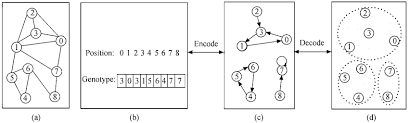
\includegraphics[scale=1.]{images/locus_img.png}
	\end{center}
	\caption{An example of the locus adjacency representation and decoded solution.}
	\label{locus_img}
\end{figure}
The second, more recent representation is called the \textit{locus adjacency representation}. It is a true graph based approach, as it relies on the topology of the network to enforce its structure. Each allele takes on an integer value, between 0 and $n$, where $n$ is the number of genes in the chromosome, which follows to be the number of nodes in the graph. The individual is not evaluated directly, but instead encodes a partitioning which can be extracted using a linear time decoding algorithm, described in \ref{locus}. The allele values give a path, from node to node, which produce a collection of subgraphs, each being a community. Figure \ref{locus_img} gives an example of a locus and its decoded solution. This representation comes with the condition that for the gene $i$ of solution $S$, $S_i$ to hold a value of $j$, nodes $i$ and $j$ must share and edge. A benefit of this condition is that any combination of individuals, representing the same graph, will yield a valid new individual.

\begin{figure}[!htb]
	\begin{center}
		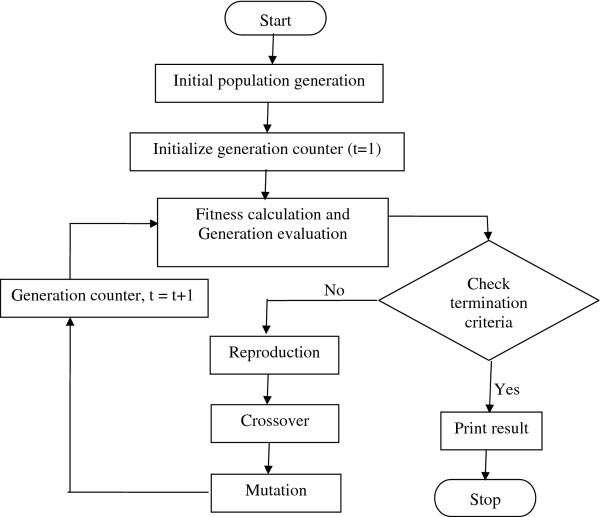
\includegraphics[scale=.5]{images/genetic_typical.png}
	\end{center}
	\caption{The flow of a typical genetic algorithm.}
	\label{logo}
\end{figure}

\begin{table}[b]
\caption{Locus Decoding Algorithm}
\label{algorithmX}
\begin{verbatim}
Decode() {
    current_c = 1
    cluster_assign = int[N]
    prv = int[N]
    for(i in 1 to N){
        cluster_assign = -1
    }
    for(i in 1 to N){
        ctr = 1
        if(cluster_assign[i] == -1){
            cluster_assign[1] = current_c
            neighbour = locus[i]
        }
    }
}
\end{verbatim}
\end{table}
